%% LyX 2.1.4 created this file.  For more info, see http://www.lyx.org/.
%% Do not edit unless you really know what you are doing.
\documentclass[english]{article}
\usepackage[T1]{fontenc}
\usepackage[latin9]{inputenc}
\usepackage{geometry}
\geometry{verbose,tmargin=1in,bmargin=1in,lmargin=1in,rmargin=1in,headheight=1in,headsep=1in,footskip=0.5in}
\usepackage{babel}
\usepackage{graphicx}
\usepackage{algorithm}
\usepackage{algpseudocode}
\usepackage{pifont}
\usepackage[parfill]{parskip}
\newif\ifdraft
\drafttrue
\ifdraft
\usepackage{xcolor}
\definecolor{ocolor}{rgb}{1,0,0.4}
\newcommand{\onote}[1]{ {\textcolor{ocolor} { (***Ole: #1) }}}
\newcommand{\terminology}[1]{ {\textcolor{red} {(Terminology used: \textbf{#1}) }}}
\newcommand{\owave}[1]{ {\cyanuwave{#1}}}
\newcommand{\jwave}[1]{ {\reduwave{#1}}}
\newcommand{\alwave}[1]{ {\blueuwave{#1}}}
\newcommand{\jhanote}[1]{ {\textcolor{red} { ***shantenu: #1 }}}
\newcommand{\alnote}[1]{ {\textcolor{blue} { ***andreL: #1 }}}
\newcommand{\amnote}[1]{ {\textcolor{blue} { ***andreM: #1 }}}
\newcommand{\smnote}[1]{ {\textcolor{brown} { ***sharath: #1 }}}
\newcommand{\pmnote}[1]{ {\textcolor{brown} { ***Pradeep: #1 }}}
\newcommand{\msnote}[1]{ {\textcolor{cyan} { ***mark: #1 }}}
\newcommand{\mrnote}[1]{ {\textcolor{purple} { ***melissa: #1 }}}
\definecolor{orange}{rgb}{1,.5,0}
\newcommand{\aznote}[1]{ {\textcolor{orange} { ***ashley: #1 }}}
\definecolor{dandelion}{cmyk}{0,0.29,0.84,0}
\newcommand{\mtnote}[1]{ {\textcolor{dandelion} { ***matteo: #1 }}}
\newcommand{\gpnote}[1]{{\textcolor{green} {***giannis: #1}}}
\newcommand{\note}[1]{ {\textcolor{magenta} { ***Note: #1 }}}
\else
\newcommand{\onote}[1]{}
\newcommand{\terminology}[1]{}
\newcommand{\owave}[1]{#1}
\newcommand{\jwave}[1]{#1}
\newcommand{\alnote}[1]{}
\newcommand{\amnote}[1]{}
\newcommand{\athotanote}[1]{}
\newcommand{\smnote}[1]{}
\newcommand{\pmnote}[1]{}
\newcommand{\jhanote}[1]{}
\newcommand{\msnote}[1]{}
\newcommand{\mrnote}[1]{}
\newcommand{\aznote}[1]{}
\newcommand{\mtnote}[1]{}
\newcommand{\note}[1]{}
\fi
\begin{document}

\title{Experiments Report}

\maketitle

\begin{abstract}
This report will include the discussion for the experiments. The experiments section will have
data plotting and an initial analysis (model and discussion) based on the developed understanding. 
A Q \& A subsection will follow after the discussion. I will add questions there that still need answering.
It would be nice if others contributed with questions!
\end{abstract}

%\begin{itemize}
%	\item
%	\begin{itemize}
%		\item
%		\item
%		\item 
%		\item 
%		\item 
%		\item 
%		\item
%\end{itemize}


%\begnn{table}[t]
%\centering
%\begin{tabular}{|p{1.6cm}|p{1.6cm}|p{1.6cm}|p{1.6cm}|} \hline
%Property 				  &CPPTraj (RMSD) &Hausdorff Distance &Leaflet Finder\\ \hline
%Single Data Scan      	  &		   &                        & \\ \hline
%Iterative      			  &No 	   &No     &Connected Components \\ \hline5
%
%All-Pairs      			  &No      &Yes          &Pairwise Distance  \\ \hline
%Intermediate Data/Shuffle &Medium  &No Shuffling       & \\ \hline
%Output Data Volume        &Low	   &Low        & \\ \hline
%\end{tabular}
%\caption{Advanced Analytics Application Characteristics}
%\end{table}

%\begin{figure}[t]
%  \includegraphics[width=.45\textwidth]{figures/CPPTrajExecutionSchematicSingleTrajectory.jpg}\quad
%  \caption{}
%  \label{fig:}
%\end{figure}

\section*{CPPTraj RMSD}
The data reported are CPPTraj comparing experiments between Vanilla (MPI) execution and the task parallel execution of CPPTraj via RADICAL-Pilot. The experiments setup is the following:

\begin{itemize}
\item RMSD over 160000 frames as a single trajectory and as an ensemble of 2 trajectories that contain 80000 frames each. (105GB filesize)
\item RMSD over 320000 frames as a single trajectory and as an ensemble of 4 trajectories that contain 80000 frames each. (209GB filesize)
\item RMSD over 640000 frames as a single trajectory and as an ensemble of 8 trajectories that contain 80000 frames each. (418GB filesize)
\end{itemize}

The configuration was from a core per 80000 trajectories up to a node per 80000 frames. All experiments were done on Stampede.

\begin{figure}[H]
\centering
  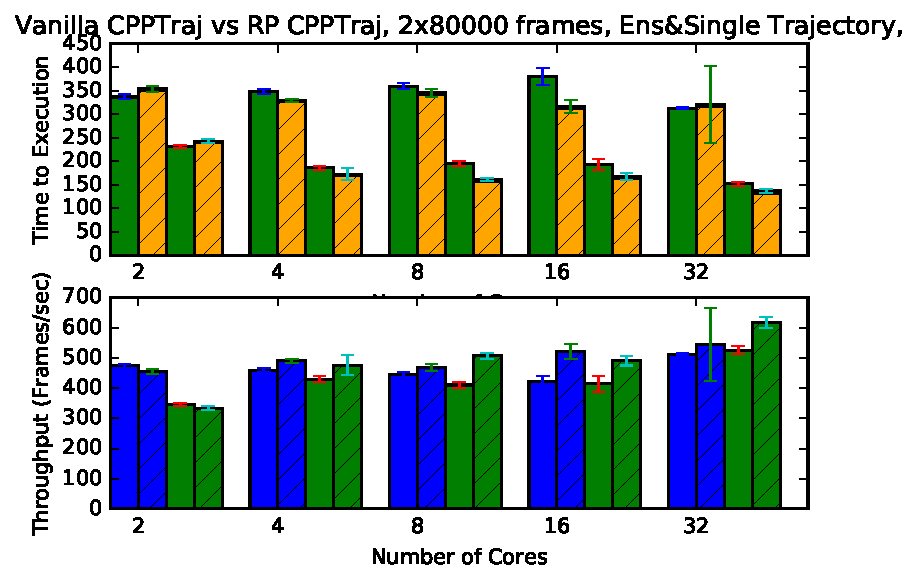
\includegraphics[scale=.70]{cpptraj/cpptrajcomparison_160Kframes.pdf}
  \caption{Time to Execution and Throughput comparison between different ways of executing the same 
  CPPTraj analysis. There are in total 160K frames organized as a single trajectory file for the 
  Single trajectory case and as an ensemble of 2 trajectories for the ensemble case}
  \label{fig:cpptrajcomparison_160Kframes}
\end{figure}

\begin{figure}[H]
\centering
  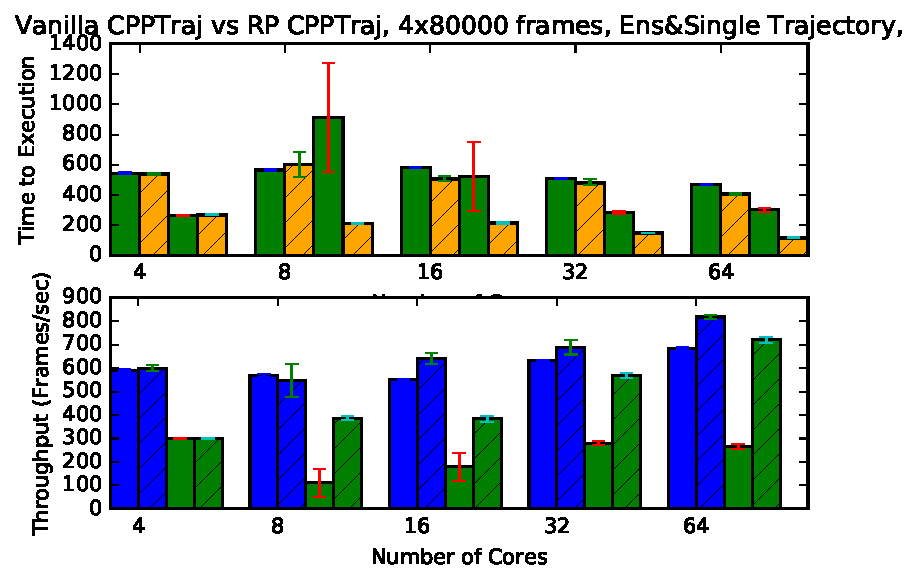
\includegraphics[scale=.70]{cpptraj/cpptrajcomparison_320Kframes.pdf}
  \caption{Time to Execution and Throughput comparison between different ways of executing the same 
  CPPTraj analysis. There are in total 320K frames organized as a single trajectory file for the 
  Single trajectory case and as an ensemble of 4 trajectories for the ensemble case.}
  \label{fig:cpptrajcomparison_320Kframes}
\end{figure}

\begin{figure}[H]
\centering
  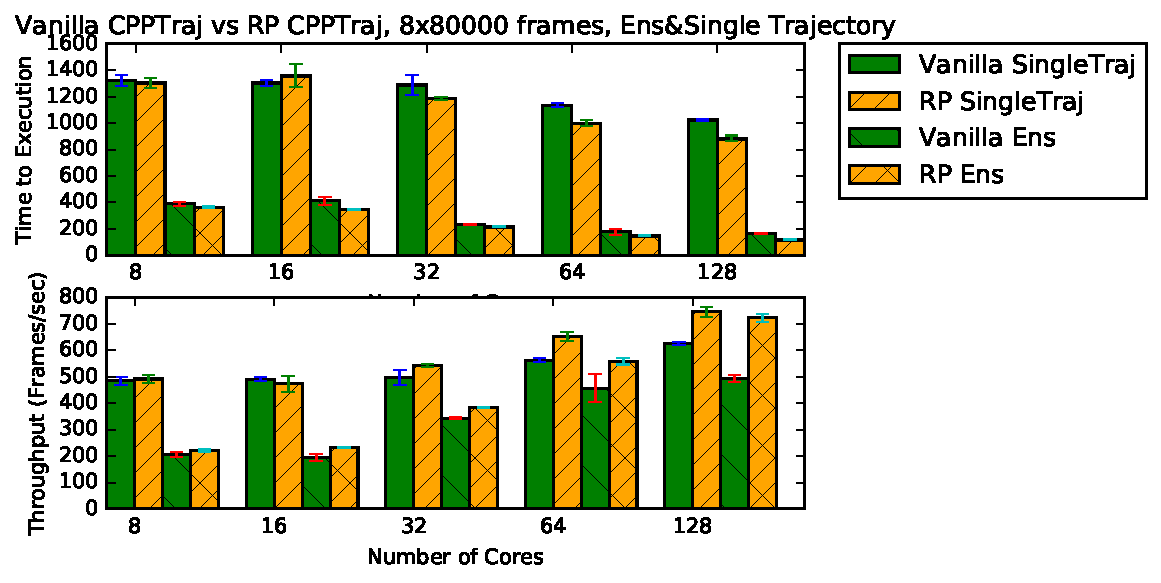
\includegraphics[scale=.70]{cpptraj/cpptrajcomparison_640Kframes.pdf}
  \caption{Time to Execution and Throughput comparison between different ways of executing the same 
  CPPTraj analysis. There are in total 640K frames organized as a single trajectory file for the 
  Single trajectory case and as an ensemble of 8 trajectories for the ensemble case.}
  \label{fig:cpptrajcomparison_640Kframes}
\end{figure}

\gpnote{The Throughput for the Ensemble Cases is for one Ensemble member. The figures need to be updated}

The top subplot show the Execution time for Vanilla and RADICAL-Pilot. The bottom
subplot shows the Average Throughput. In all figures  the order of the bars is from 
right to left:
\begin{itemize}
\item[1] Single Trajectory Vanilla, 
\item[2] RP-CPPTraj single trajectory,
\item[3] CPPTraj Vanilla Ensemble and 
\item[4] RP-CPPTraj Ensemble
\end{itemize}  

One important note to make, is that as the core count increases, the MPI implementation does not scale in 
ensemble case as the task level parallel for the 320K, Figure \ref{fig:cpptrajcomparison_320Kframes}, and 
640K frames, Figure \ref{fig:cpptrajcomparison_640Kframes}. The main difference between those two is that 
the CPPTraj execution via RADICAL-Pilot introduces a small delay between the launching of each CPPTraj 
process. I believe that this delay reduces the strain CPPTraj's MPI implementation puts to the filesystem 
and the data are read faster. In the next set of experiments with RMSD, I want to find the filesize, or 
better the system size, where the MPI implementation cannot scale anymore and the task level parallel 
can.

The reason behind the above statement is the fact that throughput remains relatively stable. 
Throughput, here measured as frames per second, is the amount of computed data per time unit. We 
can say it is the computation velocity. Throughput is a function of input rate and the number
of computing blocks. By computating blocks, I mean a self contained element that takes an input, does 
some sort of processing on the input and gives an output. In this case,it can either be a MPI process 
or a task.

Assuming that the input rate, throughin, is infinite and it can feed continuously and steadily any number of 
computing blocks, the throughput will increase linearly as we increase the number of computing blocks.
Say that such a block can process $N$ inputs per time unit. Adding a second computing block $2N$ 
inputs per time unit can now be processed. Thus, with $K$ computing blocks the throughput is $KN$ inputs 
per time unit. It is now established how throughput changes when the computation blocks vary and the input rate
is large enough to accomodate any number of them. 

Assume now that the input rate is finite to a maximum of $M$ inputs per time unit. In case $M < N$, throughput
is dectated by the input rate. In case $M \geq N$, throughput will increase linearly as long as the number
of computing blocks is less or equal to $\lfloor\frac{M}{N}\rfloor$. When the number of computing blocks,
becomes larger than the previous number, throuput flats to a rate equal to the rate in which the input is produced.

The question that needs to be answered now is what is the rate that CPPTraj reads in data. The experiments will read
the file and do nothing else. 

\end{document}
